\epigraph{If you can't solve a problem, then there is an easier problem you can solve: find it.}
{\textit{George Pólya}}
% Include an example of how to understnad someting?
% Also cover things like comparing yourself to others and why that's not always useful? 

% Address the importance of strugling with problems - build onto the workshop section from before 

\section{Building the Toolkit}

% Talk about buildling that problem solving tooklit - then link to making notes? 

In this chapter, I want to challenge the idea that a Maths degree is just about learning more advanced techniques. 

If there’s one thing worth holding on to while studying mathematics, it’s that every definition, theorem, and technique exists because someone, at some point, was trying to solve a problem.

When you first meet a new topic, it can feel like a wall of definitions followed by results you’re expected to accept and apply. But mathematics did not begin as a fixed collection of rules. It began with curiosity. The ideas you learn were built to understand patterns, resolve contradictions, and make sense of problems that genuinely puzzled people. What you usually see at university is the finished structure, not the messy exploration that led to it. You won’t always see the motivation straight away and that’s normal. But it’s still worth remembering that the mathematics you’re learning exists because someone cared enough about a problem to keep thinking about it.

And in a way, that is what you are stepping into when you study mathematics. What this degree really develops is how you respond when you don’t immediately know what to do. It’s training you to sit with uncertainty without panicking, to break a large problem into smaller parts and identify structures where none seems obvious in the first glance. 

% If there's anythign you remember... rememebr that you do.. every theorem or formula you come across is because it was trying to solve some problem.. it’s not out of nowhere.. and once you think about maths as tools for solving problems.. intuition just falls out relatively easily… mathematician in the past had a reason ot be engaged in the problems, it wasn’t out of nowhere… so everything that you learn has a reason and has motivated people in the past.. that doesn’t mean you will appreciate all of them the same way ppl in the past did, but it does give you some reason and motivation to pursue studying this beautiful subject. 


When faced with something unfamiliar, mathematics teaches you to ask: 
\begin{itemize}
    \item What do I actually know? 
    \item What is the definition here? 
    \item What would have to be true for this to work? 
    \item Can I test a simpler example with numbers before generalising it? 
\end{itemize}


\subsection{Notes That Actually Help}
% Short-mid rant on what works/has worked in the past 
% Talk a bit about my own experience with note-taking?
% Depends on person, so encourage them to try something, see how useful that's been 
% best indicator usually - if you can explain it to someone else 
% sit down with the mindset that you will learn something new - and find that thing - treat lectures like exploration, because mathematics is exploration. 

You might spend the first few weeks trying to find the `right' way to take notes for something like Mathematics. Some people swear by handwriting because it slows them down, others type in \LaTeX \ or something else because it might be neater and easier to organise, some annotate the lecture slides or notes directly. There is no `one-size-fits-all' here. What works brilliantly for one person might be useless for another. 

The only reliable test is whether the system helps you think critically or not. If you find yourself with beautiful notes on the most recent Calculus lecture you attended but have no idea on how to approach the problem sheet, something needs to change. If you find not making any notes in lectures and reviewing information later in the evening helps ideas settle, try that. Or if you realise handwriting slows you down, see if you can find a way to condense information instead of copying a lot of things down. 

The goal here is not to produce the most elegant looking notes amongst your peers, but to build understanding that you can use for yourself. You are not being graded on your notes, but on your thinking, so ensure that the learning resources you use/build contribute to your thinking. 

\subsection{Explaining Things Out Loud}
% cite/reference the 'feynman' technique in the margin or something?

One habit that has helped me more than any particular note-taking method was explaining things out loud. 

A good test to see if you've understood something is usually later in the day or in the week, close your notes and try to explain the main idea either to a friend or out loud. 

You very quickly discover what you don't understand when you try to speak it. On paper, everything can look fine. But the moment you try to explain why some assumption is necessary, or why an implication follows, you feel the gap immediately. If you can explain a concept to someone else, even to an imaginary audience without constantly checking your notes, you are much closer to understanding a concept than if you simply reproduce what was written in the lecture. 
 

\section{What to Do When You're Stuck}

Problem solving sounds very inspiring until you're staring at Question 4 from Coursework 2 at 10:37pm or 38 minutes into the exam and your brain has gone offline. There will be moments in lectures or problem sheets or exams where you may genuinely not know how to begin. 

The instinct when stuck is often to rush, to scan the question faster or hope something jumps out. Instead, try and slow down. Read the question again. What is actually being asked? Rewrite the question in simpler terms and alongside it, any definitions or theorem you can recall about what is being asked. This does two things. First, it forces your brain back into structure and something you do know rather than panic. And secondly, everything that you need is given to you in the words of the question, and once you have unpicked the most important parts, you have part of a path forward. 

\section{On Gaining Insight}
% Need example of when I was really stuck on stuff 
\begin{quote}
One of the hardest things to unlearn at university is the urge to look at a solution the moment you feel stuck. Once you've seen someone else's solution, you can never recreate the benefit of discovering it yourself. Even if you don't solve the problem completely, struggling with it, forming wrong ideas, testing different approaches and hitting multiple dead ends does far more for your mathematical growth than neatly following a polished answer ever will.
\end{quote}

To illustrate this with an example, I remember getting stuck on a problem in my Linear Algebra II module that, in hindsight, was conceptually quite simple: showing that a certain set of functions formed a vector space. The technical details are not that important here.

On the one hand, I could've easily looked up the proof or asked AI to generate it in a few seconds, and it would probably have given me something correct and tidy. It might even have felt satisfying in the moment, but I suspect I would have mostly walked away with the illusion of understanding. 

Instead, I was in the workshop where I had my lecturer from the module present to talk me through the problem and refine the gaps in my thinking. Rather than being simply told what I had to write for the proof to fall out, we started from what I did know about the definition of additive identity and what it was supposed to satisfy, namely the condition $f +0 =f$, then treated this like an equation and worked out what this mysterious `zero function' would look like. 

Arriving at that idea, and more importantly, learning how to justify it properly, was the real insight. But that insight didn't come from seeing the finished proof, but from wrestling with the gap between knowing the definition and knowing how to write it in the abstract way the questions asked me to. Now, if I had skipped that part and just read up the solution, I would have `known' the answer, but would have lost the experience of learning how to reconstruct that kind of proof myself. 

And that's the difference. When you outsource your thinking, you might take pride in being incredibly efficient. But the price of efficiency is ownership, and the price of speed is insight, and with a subject as elegant and satisfying like Mathematics, that trade is just not worth it. 

\section{Why This Matters}

This reason these problem solving skills matter is not because you will be constantly proving theorems outside university. It matters because the habits transfer. Learning how to decompose complex problems into manageable parts, staying calm under uncertainty, testing assumptions, communicating reasoning clearly. These are all thinking skills that reshape how you approach problems in the real world. 


\begin{figure}[H]
    \centering
    \begin{minipage}{0.48\linewidth}
        \centering
        
\includegraphics[width=\linewidth]{xkcd/advancedTechniques.png}
        \caption{\textbf{\href{https://xkcd.com/2595/}{Advanced Techniques}}}
    \end{minipage}
    \hfill
    \begin{minipage}{0.48\linewidth}
        \centering
        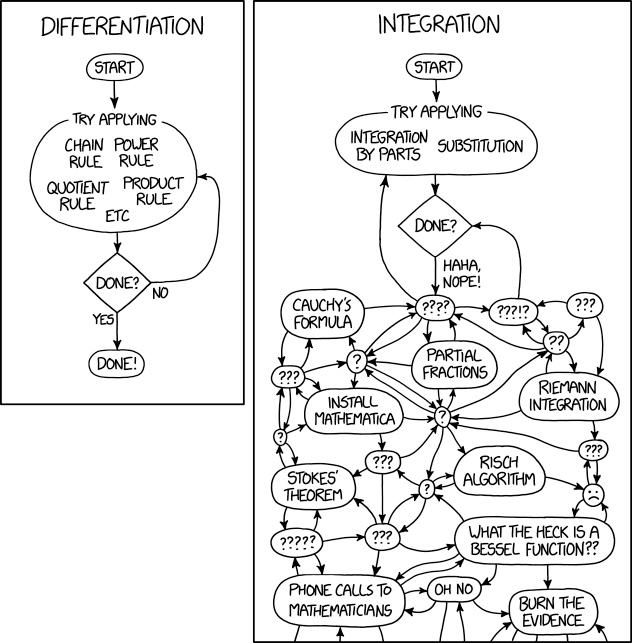
\includegraphics[width=\linewidth]{xkcd/integration.png}
        \caption{\textbf{\href{https://xkcd.com/2117/}{Differentiation and Integration}}}
    \end{minipage}
\end{figure}